\documentclass[plain]{sigplanconf}
\usepackage{balance} % For balanced columns on the last page
\usepackage{amsmath}
\usepackage[T1]{fontenc}
\usepackage{lmodern}
\usepackage{graphicx}
\usepackage{amssymb}
\usepackage{tikz}
\usepackage{array}
\usepackage{longtable}
\usepackage{subcaption}
\usepackage[
bookmarksopen,
bookmarksdepth=2,
breaklinks=true
]{hyperref}
\usepackage{natbib}
\setcitestyle{square,sort,comma,numbers}
\makeatletter
\def\BState{\State\hskip-\ALG@thistlm}
\makeatother

\makeatletter
\def\@copyrightspace{\relax}
\makeatother
\begin{document}
	\title{Community Networks QoS Monitoring System}

	\authorinfo{Clayton Sibanda}
	{Department of Computer Science\linebreak University of Cape Town\linebreak South Africa}
	{}
	\maketitle
	\begin{abstract}
	\paragraph{}
	Characterising the internet through measurements has
	become very important to both end users and network
	managers. Most end users want to know what is causing their network based applications to slow down or take too long to respond. On the other hand network managers want to troubleshoot and detect faulty nodes in a network.
	\paragraph{}
	
	\end{abstract}
	\begin{CCSXML}
		<ccs2012>
		<concept>
		<concept_id>10003033.10003079.10011704</concept_id>
		<concept_desc>Networks~Network measurement</concept_desc>
		<concept_significance>100</concept_significance>
		</concept>
		</ccs2012>
	\end{CCSXML}
	\ccsdesc[100]{Networks~Network measurement}
	\keywords
	Community Networks, Data-driven Networking, Quality of Services
	
\section{Background}
\paragraph{}
An network/internet measurement platform is an infrastructure of dedicated probes that periodically run network measurement tests on the internet/network\cite{7076582}.

\paragraph{}
 Network measurement platforms from the perspective of end systems normally play an important role both for researchers who want to develop general insight into how the Internet functions, and for general practitioners who want to diagnose individual performance issues \cite{Dhawan:2012:FBN:2398776.2398786}. Use cases of these measurement platforms vary widely based on the type of a user and the end goal of the measurement \cite{Ford:2018:RWR:3243157.3243167}. One example of a use case is how in  previous studies these platforms have been employed to understand the overall network topology of the internet\cite{7076582}.
\paragraph{}
For managers and regulators measurement platforms can provide a different view of the internet e.g routing, topology, addressing and naming, security, dataplane performance or impairment and traffic matrices\cite{Ford:2018:RWR:3243157.3243167}.
\paragraph{}
In some cases these platforms are used to detect anomalous behaviour in the network which could be caused by users abusing the network or general cyber attacks. Internet service providers(ISP) on the other hand use monitoring platforms to evaluate the Quality of Service(QoS) experienced by their users\cite{7076582}. Consumers can also use such measurements to confirm whether the ISP is living up to its Service-Level Agreement(SLA) offers \cite{7076582}.
\paragraph{}
In general measurement platforms are said to provide the engineering to bridge the gap between practice and research in terms of coordination to allow a measurement to scale  and representation producing simple and useful results \cite{Ford:2018:RWR:3243157.3243167}.
\subsection{Quality Of Service}
Quality of Service(QoS) is concerned about the network
delivery capacity and resource availability to users\cite{5430142}. In
other words one would say QoS is about fast internet
access for the user and low latency. 
\paragraph{}
However there are many non-uniform views about QoS by different
stakeholders. Some say QoS refers to the ability of the
network to offer packet transfer in a faster way \cite{5430142}.
\paragraph{}
At the same time other organisations have maintained that
QoS has to do with the degree of conformance to user-specified needs \cite{article}. These two different views raise questions of how network level QoS measurements and control relate to the user perception of a service \cite{5430142}.
\paragraph{}
The two main QoS parameters are network latency
and delivery speed(bandwidth) \cite{5430142}. As a result QoS is
considered poor if any of them is affected from their normal position i.e if bandwidth is low or if latency is high.
\subsection{Community Networks}
Community networks are IP-based networks that are built, operated and owned by communities of citizens. These networks are sometimes ran by non-profit organisations working together with local stakeholders in the community. 

Other scholars define them as large scale, self-organized and decentralized networks, built and operated by citizens for citizens \cite{Braem:2013:CRC:2500098.2500108}.
\paragraph{}
These networks are normally built as a mixture of both wireless and wired links. This calls for different routing and systems and protocols to be employed in these networks. In some cases there many wireless links with a limited number of wired links. This makes them predominantly wireless networks\cite{Braem:2013:CRC:2500098.2500108}.
\paragraph{}
Providing connectivity to community networks can be a challenging task since nodes use diverse access technologies and display a great deal of mobility \cite{Plagemann2008}.
Due to their non-standard architecture and the use of diverse technology it has proven to be difficult to deploy conventional network measurement platforms on community networks.


\section{Introduction}
	\paragraph{}
Characterising the internet through measurements has become very important to both end users and network
managers. Most end users want to know what is causing their network based applications to slow down or take too long to respond. On the other hand network managers want to troubleshoot and detect faulty nodes in a network. The rise of cyber attacks and abuse of networks also makes it of paramount importance for network managers to continuously keep track of what is happening in their network.
\paragraph{}
The goal of this is to present the design and creation of a visualiser for a quality of service monitoring platform for community networks. Such a visualiser is important in that it can help in monitoring network activity and identifying anomalous behaviour.
\paragraph{}
The platform is built as case study for the iNethi community network at ocean view. There are two main types of target users for this platform. The first ones are non-technical end-users of the network. These are people who live in the community and use the network for different purposes. The second group are technical(advanced) end-users with a working knowledge of networking protocols. These would include networking researchers from tertiary institutions and network managers.
\paragraph{}
For non-technical users, the goal of the platform is to enable them to get various statistics calculated based on their past network usage. These statistics will also include websites or services which consumes most of their data and the services they visit the most.
\paragraph{}
On the other hand, the goal for technical users, is to allow them run different measurements on the network with intention to monitor network activities. The results of the measurements are to be displayed on a rich web based visualiser that employs interactive graphs to present each type of measurement. These measurements are to be run on a number of mobile probes deployed haphazardly on the network. Fig 1 shows how the whole system is to be connected together.

\begin{figure*}
	\centering
	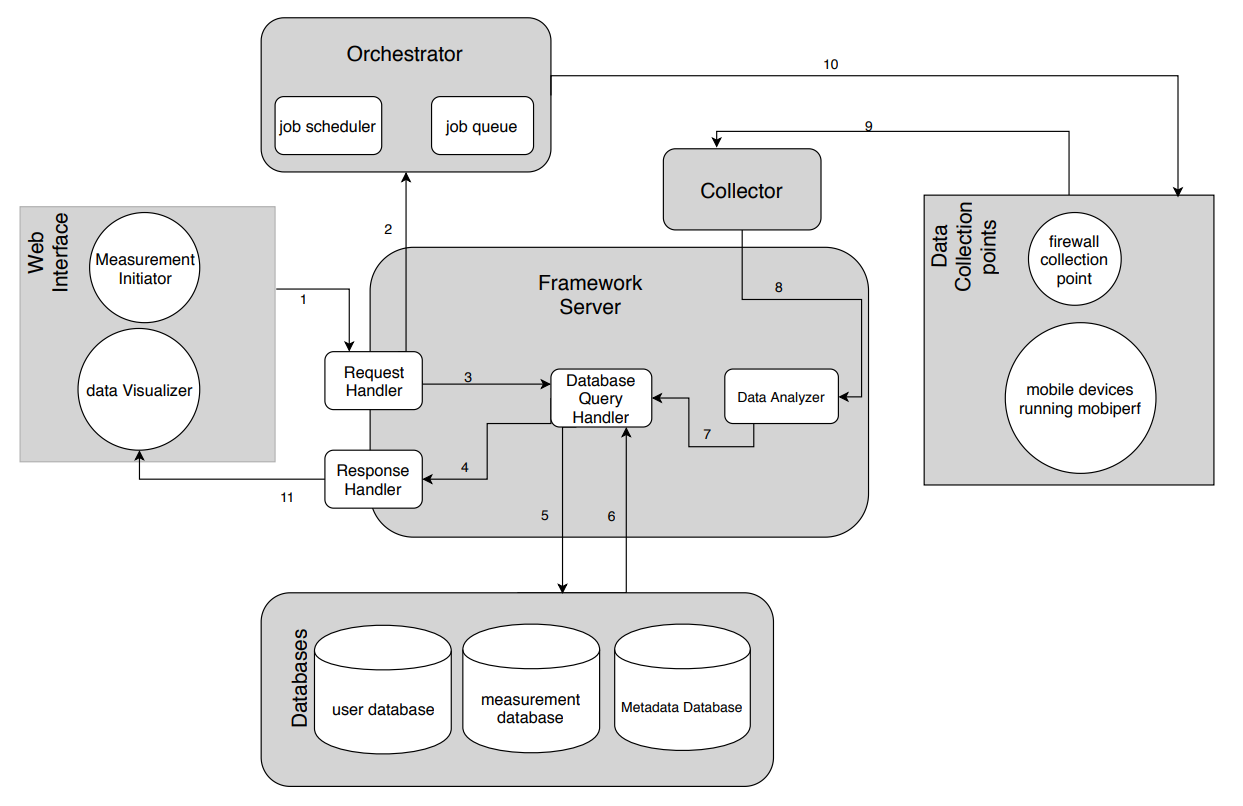
\includegraphics[width=0.7\linewidth]{images/system}
	\caption{Image of the system showing how the visualiser was connected to everything}
	\label{fig:system}
\end{figure*}
\input{sections/background}
\section{Literature Review}
\subsection{Prominent network measurement platforms}
There are a number of network measurement software
that are currently deployed to monitor and observe patterns in different networks.
\paragraph{}
The first one that we discuss is PerfSONAR(Performance focused
Service Oriented Network monitoring ARchitecture)\cite{10.1007/11596141_19}. This is a service infrastructure that is web based and is used to collect and publish network performance monitoring\cite{article2}. Its main goal is to make it easy to handle end-to-end performance problems on paths going through several networks \cite{article2}. It does this by using a set of services to deliver performance measurements to an agreed upon network environment.

\paragraph{}
LiveLab is a method used to measure smartphone usage in the field and to measure wireless networks through smartphone users\cite{article3}. This platform employs a tool that is custom built for Iphones only to enable researchers to track users in the field. LiveLab also provides a comprehensive in-device logging of smartphone usage and measurement of wireless
networks\cite{article3}.The tool takes advantage of the mobility
of users and the ability of smartphones to switch connections between multiple routers and that way researchers are able to gain large amounts of data\cite{article3}.

\paragraph{}
RIPE ATLAS is also another tool used extensively
to measure network performance. It uses thousands of
distributed probes and anchors as measurement devices.
The tool can perform IPv4 and IPv6 traceroute, ping,
DNS, NTP\cite{7076582}.
\paragraph{}
PlanetLab is a measurement platform used for testing of new network services. However PlanetLab is rather unusable due to unpredictable load issues and tendency of nodes to be located in a national research network\cite{7076582}.
PeerMetric is a measurement tool used to measure P2P network performance experienced by broadband hosts\cite{7076582}.
\paragraph{}
Mobiperf is an android based application that is used to collect mobile network measurements. On the backend it uses a data collection server to collect and aggregate data. The app periodically checks in with the measurement server which sends it a list of measurement tasks to perform. These measurement tasks include ping, trace-route, HTTP GET, DNS lookup, TCP Throughput, IPv4/v6 compatibility check and UDP Burst. Each task is given a respective set of measurement parameters.

\subsection{ Challenges with network measurement platforms}
In some previous studies measurement platforms have been observed to bring about challenges in the into the network.
\paragraph{}
One of the most common major challenge is the fact that integrating a platform into a system can bring about cyber security risks. This because some measurement platforms might need admin privileges for them to carry out some measurements. This opens the network into a lot of privacy risks.

\subsection{Visualisation}
Networks today generate large volumes of data due to a lot of people getting connected to the internet. The numeric nature of such data which consists of packet size, time and other statistical features makes it hard to perceive relationships between the data\cite{Ruan2018}. According to a paper by Ruan et al.[2018], visualisation has proven to be a very imperative tool to capture and display network activities. In some cases visualisation has also made it easy to detect and prevent cyber security threats in the network\cite{inproceedings}.
\paragraph{}
There are a number of visualisation techniques that are currently used to capture network data. These include pie charts, line graphs and histogram which are the core visualisation methods. However these are not effective for network data which contains more two dimensions\cite{Ruan2018}. Multi-dimensional visualisation methods include scatter plot, hyper graph, force graph and parallel coordinate. Due to the limitation of human vision there is need for dimensionality reduction to be done before visualisation\cite{Ruan2018}. 
\paragraph{}
The most popular algorithm for dimensionality reduction is principal component analysis(PCA) which implements dimensionality reduction by deriving new features. PCA has multiple applications but also has its own drawbacks, by reducing dimensions we lose some information in the dataset\cite{Ruan2018}.







\section{Design and Implementation}
\subsection{Approach}
The purpose of a network visualiser is to allow users to analyse and get insight into how they use the network\cite{Ruan2018}. It also allows network managers(advanced users) and researchers to schedule and perform measurements. The results of the measurements are also displayed on interactive graphs for further analysis.
\paragraph{}
For this project an iterative user-centred design(UCD) approach was adopted. This entails that the user is involved throughout the whole design process so that the visualisation produced meets every need that the user has\cite{Andrews:2006:EIV:1168149.1168151}. The goal of this approach is to find out the needs and tasks of the user and then design based on that\cite{Dylggduu}. This visualisation platform is developed for a system that is to be deployed at a local community network called iNethi in Cape Town. Users of this visualisation platform are expected to be network researchers, network managers and general users of the network.
\paragraph{}
This approach consisted of three phases:early envisioning phase, the global specification phase and the detailed specification phase\cite{Kulykinbook}.
\paragraph{}
The early envisioning phase entails the analysis of the users, the environment they are in and their tasks. This will enable us to profile users and gather requirements in the process\cite{Kulykinbook}. In the context of a network visualiser, the would mean understanding the type of data that user would to see visualised and analyse. A number of methods can be employed to obtain this which include surveys, interviews and focus groups\cite{Kulykinbook} \cite{Abras04user-centereddesign}.
\paragraph{}
In the global specification phase and the detailed phase, a designer comes up with a solution and presents it to users\cite{Abras04user-centereddesign} \cite{Kulykinbook}. Each phase may contain multiple iterations of design and analysis with evaluations taking place in all phases\cite{Abras04user-centereddesign}.
\paragraph{}
\begin{figure}[b]
	\centering
	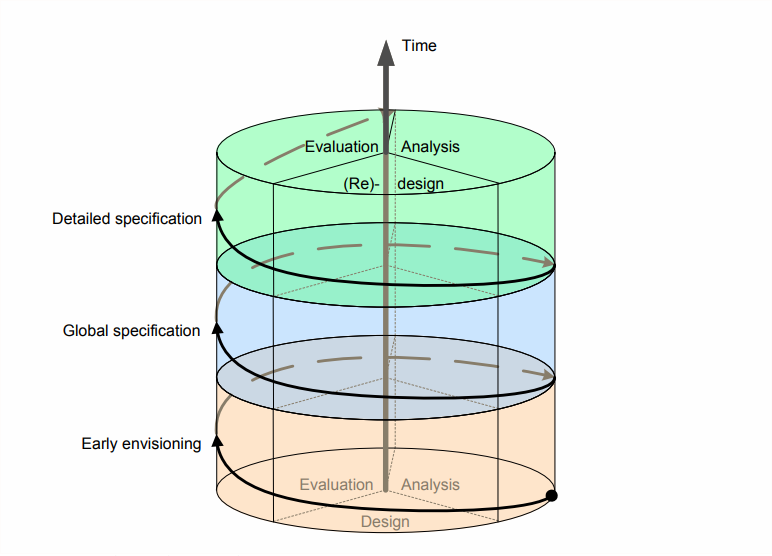
\includegraphics[width=0.7\linewidth]{img1}
	\caption{User-centered visualisation design process\cite{Abras04user-centereddesign}}
	\label{fig:img1}
\end{figure}

\paragraph{}
Users generally have different abilities and tasks to perform on the visualisation tool. Due to these differences it is imperative that a detailed analysis of the users, their environment and their tasks is performed before the design of the visualisation platform.


\section{Final evaluation and results}
\subsection{Evaluation Metrics}
The goal of the evaluation method was to asses the potential use of the web visualiser. Evaluating user experience was the best way to understand if the visualiser met the user's expectations. Feedback and suggestion given by users were taken and used to improve the effectiveness and accuracy of the visualizer\cite{lam:hal-00723057}

\subsubsection{Effectiveness and Accuracy}
In user interface design, effectiveness is used to describe the functionality of a tool and  also evaluates a user's performance when performing tasks. Accuracy on the other hand refers to the way in which data/information is presented to the user. To ensure effectiveness, a lot of affordances and feedback mechanisms were employed on the visualisation.
\subsubsection{Usability}
Usability can be described as the measure of  the quality of use of a platform/application by a potential user. This makes it an essential component of visualisation to take into account\cite{1509067}.
\paragraph{}
During usability tests, users were allowed to perform prescribed tasks while their interaction with the interface were observed, their reaction to certain tasks were also taken into account. This was done so that user task completion and tasks success rate could be measured. The main tasks to be performed were chosen based on major features.


\subsection{Usability Tests}
In order to test the effectiveness, accuracy and usability of the visualisation, usability tests were done with eight potential users. Four of these users researchers from UCT while the other four were members of the Ocean View community. 
\paragraph{}
Task completion was used to measure accuracy and effectiveness during the tests while ease of use(ability to navigate the app with ease) was used to gauge usability. A questionnaire consisting of both scales and free response questions were used to collect user feedback.
\paragraph{}
To conduct usability studies, an ethical clearance was obtained from the Department of Student Affairs and the Science Faculty Research Ethics Committee. At the beginning of the usability test, participants were asked to sign a consent form outlining the agreement between the researchers and them. The form also guaranteed them anonymity of their results.
\paragraph{}
The usability study with community member was done first. Participants did the tests individually, one at a time. After performing their tasks and providing feedback,the next user was given their set of tasks to complete which were different from the previous one. The same process was followed with researchers from UCT but with a different set of tasks that were specific to users with a working knowledge of computer networks.
\subsection{Analysis of Results}
\subsubsection{Task Completion}
The success of a task was defined by the attainment of different objectives for each task. For some other tasks it can generally be referred to the participant's ability to obtain some data during execution of a certain task. Since participants we observed while performing the task, a participant was said to be successful if they completed the task at hand.
\paragraph{}
From the results, it was observed that all users were able to complete certain tasks while others struggled with more involved tasks. The results of the  two sets of tasks are shown on Figure 6 and Figure 7.

\begin{figure}
	\centering
	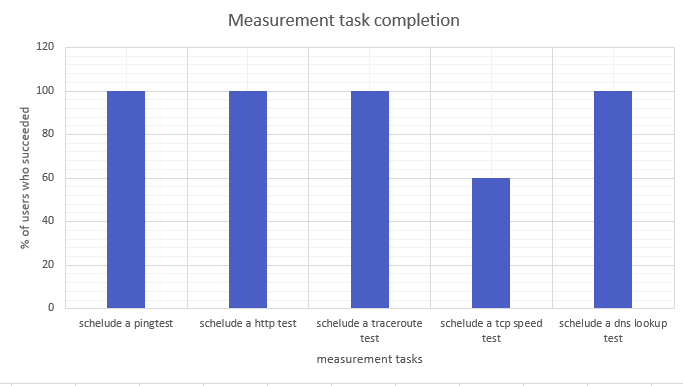
\includegraphics[width=1\linewidth]{images/task1}
	\caption{Completion rate of the first set of tasks}
	\label{fig:proto}
\end{figure}

\begin{figure}
	\centering
	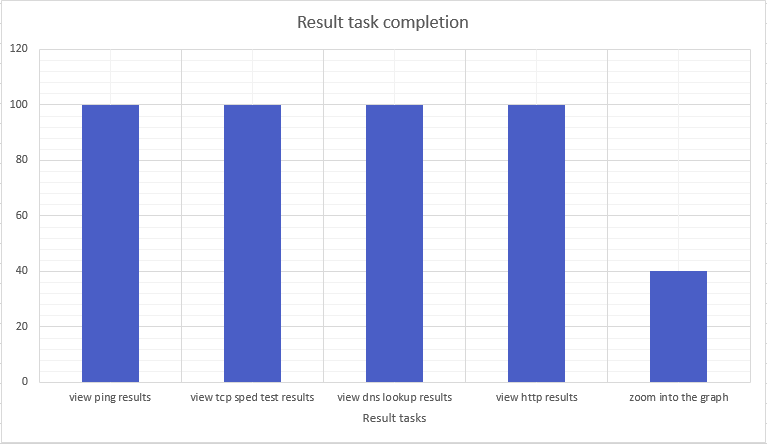
\includegraphics[width=1\linewidth]{images/task2}
	\caption{Completion rate of the second set of tasks}
	\label{fig:proto}
\end{figure}
\subsubsection{User Feedback}
A questionnaire that consisted of a scale and free response questions was given to participants  at the end of each usability test. The free response questions for researchers added were "Do you think the app provides enough information for networking researchers/network administrators?. If not what else would a user want?" and "Do you have any other feedback on the application?". This allowed users to elaborate on their experience with the application.
\paragraph{}
For the Ocean View community members, these were the free response questions "Do you think the app provides enough information for Inethi network users?. If not what else would a user of the network want?" and "What did you like the most about the app for you?".
\paragraph{}
These questions were not compulsory for participants but a significant number of them answered nonetheless. 
\paragraph{} 
The majority of researchers said that the platform provided them with information. However the common suggestion was that more parameters should be included on the graphs especially for tcp speed test.
\paragraph{}
Ocean community members also asserted to the fact the platform provided useful information to potential users. They also suggested other features which would enable one to monitor network activity of their children. 
\section{Limitations}
\section{conclusion}
In this paper, we presented the design of a quality of service monitoring platform for iNethi community network. For this design, a user centred design approach was adopted and used over two iterations(phases). The final visualisation was built as a result of the success of the previous iterations.
\paragraph{}
The visualiser consists of two parts. A measurement initiator and data visualizer. The measurement initiator allows users to schedule and run experiments on different probes while the data visualizer displays to the user the results of the measurements performed by the probes. 
\paragraph{}
On the measurement initiator, the user can schedule and run five different measurement types which are HTTP, DNS lookup, ping, traceroute and TCP speed test. The data visualizer employs interactive graphs and JSON texts to display measurement results.
\subsubsection{Future works}
Ideally the platform will need to deliver real time data to the visualiser. However this cannot be done with user's phones being used as probes. This is because the phones will have to continuously measure and send data to the server, and this may affect the user's phones. As a result, a viable probe for real-time data will be a device like a raspberry pi installed within the network.
\paragraph{}
Currently, we use email addresses for authorising users to access data and view network data. This happens to be an insecure way of authorising users. We therefore suggest the use of both an email and password to authenticate all users.
\subsection{ACKNOWLEDGEMENTS}
Thanks to project team members David Kheri and Meluleki Dube for their contributions and Dr Josiah Chavula for his guidance throughout the project as project supervisor. An additional thank you to Dr Maria Keet for her input as second reader.. 
	%\nocite{*}
	\bibliographystyle{acm}
	\bibliography{references}
%	\input{sections/appendix}
\end{document}